\chapter{Ausgewählte Aspekte}
\section{WCAG 2.1}
\label{wcag_2_1}
Die Web Content Accessibility Guidelines 2.1 (WCAG 2.1, vgl. \cite{wcag_2_1_2018}) wurden im Dezember 2008 veröffentlicht und sind ein Standard, der weltweit verwendet wird, um Dienstleistungen im Web so barrierefrei wie möglich zu gestalten. Somit können auch Menschen mit Behinderungen, wie etwa Sehschwäche, Blindheit, Hörverlust, Taubheit, körperliche oder kognitive Einschränkung, Sprachbehinderung, Lichtempfindlichkeit, Lernbehinderung oder Kombinationen dieser, das World Wide Web nutzen. Diese Richtlinien sind vom World Wide Web Consortium (W3C, vgl. \cite{w3c_1994}) am 5. Juni 2018 für Webanwendungen empfohlen worden.

Durch die Befolgung der Empfehlungen des W3C können Webdesigner und -entwickler, politische Entscheidungsträger, Käufer, Lehrer und Studenten beziehungsweise Schüler das WWW nahezu problemlos nutzen. Die WCAG 2.1 setzen sich aus allgemeinen Prinzipien, allgemeinen Richtlinien, prüfbaren Erfolgskriterien sowie einer Vielzahl an Techniken zusammen:

\begin{itemize}
	\item Es gibt vier \textbf{Prinzipien}, die die Grundlagen für die Web-Zugänglichkeit bilden: wahrnehmbar, bedienbar, verständlich und robust (englisch: perceivable, operable, understandable and robust).
	\item Die Prinzipien beinhalten insgesamt 13 \textbf{Richtlinien}, an die sich Entwickler halten sollen, um das Web zugänglicher zu machen. Sie sind zwar nicht prüfbar, helfen allerdings dabei die Erfolgskriterien besser zu verstehen und die Techniken besser umzusetzen.
	\item \textbf{Prüfbare Erfolgskriterien} werden dort eingesetzt, wo bestimmte Anforderungen und Tests für die Konformität erforderlich sind, wie etwa beim Entwurf, beim Kauf, bei Regelungen und bei vertraglichen Vereinbarungen. Es gibt drei Ebenen der Konformität, wobei die höchste AAA, die mittlere AA und die niedrigste A ist.
	\item \textbf{Ausreichende und beratende Techniken} dienen zur Erfüllung der Erfolgskriterien und als Beratung. Häufig vorkommende Misserfolge sind ebenfalls dokumentiert.
\end{itemize}

Bei Erreichung der höchsten Ebene ist eine hundertprozentige Web-Zugänglichkeit jedoch nicht garantiert. Die WCAG 2.1 dienen ausschließlich als Anleitung, um das Web so barrierefrei wie möglich zu gestalten. Deshalb wird vom W3C empfohlen sich regelmäßig über den neuesten Stand zu informieren und sich mit anderen zu beraten. Folgende Bemerkung wurde vom W3C (2008, \cite{wcag_2_1_2018}) auf der Webseite veröffentlicht:\\
``[...] Authors are encouraged to consider the full range of techniques [...] as well as to seek relevant advice about current best practice to ensure that Web content is accessible, as far as possible, to this community. [...]``

\section{Web Components}
\label{web_comp}
Web Components (vgl. \cite{moz_webcomp_2019}) sind eine Web-Technologie, die es den Entwicklern ermöglicht, selbstdefinierte HTML-Elemente zu erstellen und wiederzuverwenden. Diese sind mit ihrem CSS und JavaScript gekapselt und sind somit vollständig von anderem Code getrennt. Mit einigen JavaScript Frameworks wie etwa Angular war es zwar bereits möglich wiederverwendbare HTML-Elemente zu definieren, allerdings nutzt jedes der Frameworks einen anderen Standard. Dies bedeutet, dass der Code in anderen Projekten in den meisten Fällen nicht verwendbar ist. Genau dieses Problem wurde durch Web Components gelöst. Die Web Components bestehen aus drei Hauptbestandteilen:

\begin{itemize}
	\item \textbf{Customs ELements:} Ein Satz von JavaScript APIs zur Definition von benutzerdefinierten Elementen.
	\item \textbf{Shadow DOM:} Ein Satz von JavaScript APIs zum Hinzufügen eines DOM-Elementes mit gekapselten Shadow-DOM-Elementen, welches separat vom Hauptdokument DOM gerendert wird. Dadurch ist es möglich jegliche Funktionalitäten isoliert zu definieren, sodass der Programmierer keine Rücksicht auf Kollisionen mit anderen Dokumenten nehmen muss.
	\item \textbf{HTML Templates:} Markup-Vorlagen, die innerhalb der Elemente \texttt{<template>} und \texttt{<slot>} geschrieben werden, werden nicht auf der dargestellten Seite abgebildet. Diese sind dafür da, um sie mehrmals als Vorlage eines benutzerdefinierten Elements zu verwenden.
\end{itemize}

% Factory Pattern, Events, Delegate, Observer
\section{Factory Method Pattern}
\subsection{Was sind Design Patterns?}
Um das Factory Method Pattern zu verstehen, muss man zunächst einmal wissen, was ein Design Pattern (dt. Entwurfsmuster, vgl. \cite{design_pattern_2020}) ist. In der Softwareentwicklung treten beim Entwurf oftmals dieselben Probleme auf. Abhilfe hierfür schaffen Design Patterns, die eine allgemeine wiederholbare Lösung dieser Designprobleme sind, den Entwicklungsprozess beschleunigen und programmiersprachenunabhängig sind. Sie repräsentieren somit eine Idee, und keine spezielle Implementierung, durch deren Verwendung der Quellcode flexibler, wiederverwendbar und einfacher für die Entwickler zu warten ist. Allerdings sind sie nicht in jedem Projekt zwingend erforderlich, da sie lediglich für die Problemlösung und nicht für die Projektentwicklung gedacht sind.

\paragraph{Arten von Design Patterns}\mbox{}\\

\begin{itemize}
	\item \textbf{Creational Pattern (dt. Erzeugungsmuster):} Sie dienen dazu Objekte zu erzeugen. Dieser Prozess wird gekapselt und ausgelagert, sodass die Objekterzeugung von der Implementierung des Objektes klar getrennt wird.
	\item \textbf{Structural Pattern (dt. Strukturmuster):} Sie stellen vorgefertigte Vorlagen für die Beziehungen zwischen den Klassen zur Verfügung und erleichtern somit den Softwareentwurf.
	\item \textbf{Behavioral Pattern (dt. Verhaltensmuster):} Sie führen dazu, dass die Software flexibler wird, indem das komplexe Verhalten dieser Software modelliert wird.
\end{itemize}

\subsection{Begriffserklärung und Verwendung}
Das Factory Method Patten (vgl. \cite{factory_method_2020}), auch bekannt als Factory Pattern oder Fabrikmethode, definiert ein Interface oder eine abstrakte Klasse zur Erstellung von Objekten. Die Objekterstellung wird hierbei von den Subklassen übernommen, die entscheiden welche Klasse instanziiert wird.

\begin{figure}[H]
\begin{center}
	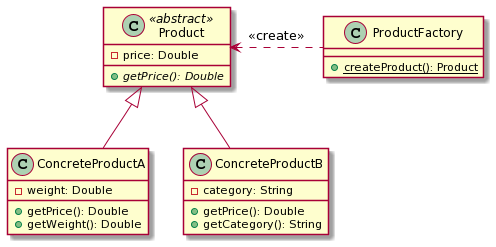
\includegraphics[scale=.7]{images/cld_factory_pattern.png}
\end{center}
	\caption{Veranschaulichung des Factory Method Patterns in einem Klassendiagramm}
\end{figure}

\subsection{Vorteile und Nachteile}
\paragraph{Vorteile}

\begin{itemize}
	\item Mit Hilfe des Factory Method Patterns können Unterklassen die Art, wie Objekte erstellt werden sollen, selbst wählen.
	\item Dieses Design Pattern fördert die lose Kopplung. Das heißt im Allgemeinen, dass anwendungsspezifische Klassen 			nicht mehr in den Code eingebunden werden müssen. 
	\item Die Kommunikation erfolgt ausschließlich über die Schnittstelle oder die abstrakte Klasse, so dass der Code mit allen 		Klassen funktioniert, die entweder die Schnittstelle implementieren oder die abstrakte Klasse erweitern.
\end{itemize}

\paragraph{Nachteile}

\begin{itemize}
	\item Falls die verwendeten Klassen nicht abstrakt sind, muss für jede individuelle Klasse eine Factory geschrieben werden.
\end{itemize}

\section{JavaScript Events \& EventListener}
\paragraph{trix-initialize}\mbox{}\\
Sobald der \texttt{<trix-editor>} im DOM registriert wird und sein internes \texttt{Editor}-Objekt zur Benutzung bereit ist, wird das Event \texttt{trix-initialize} gefeuert.\\
Damit nicht die standardmäßig definierte Toolbar, sondern die erweiterte barrierefreie Toolbar, die diese ersetzen soll, angezeigt wird, ist es möglich auf dieses Event zu hören und dementsprechend darauf zu reagieren. Somit kann mit der Trix-Extension die Toolbar ersetzt werden, ohne dass der Endbenutzer etwas von diesem DOM-Manipulationsprozess mitbekommt. % TODO: Formatierung

\paragraph{mousedown}\mbox{}\\
Das \texttt{mousedown} Event wird genau zu dem Zeitpunkt gefeuert, an dem sich der Mauszeiger auf einem HTML-Element befindet und dieses drückt.\\
Damit ein HTML-Button in der \texttt{<trix-toolbar>} aktiv ist und geklickt werden kann, hört dieser standardmäßig auf ein \texttt{mousedown} Event. Um diese Buttons mit einer Tastatur bedienen zu können, müsste der Trix-Editor im Quellcode auf Tastatureingaben reagieren und diese dementsprechend erneut validieren. In der Erweiterung Trix-Extension wird dieses Event künstlich ausgelöst mit \texttt{EventTarget.dispatchEvent()} und somit sind die Buttons in der Toolbar auch über die Tastatur bedienbar, ohne dass der Quellcode mit Wiederholung der Validation ergänzt werden muss.

\paragraph{keydown}\mbox{}\\
Wenn eine beliebige Taste gedrückt ist, wird das \texttt{keydown} Event gefeuert und liefert einen Code, der aussagt, welche Taste im Moment gedrückt wird.\\
Um den WYSIWYG Texteditor mittels einer Tastatur bedienen zu können, wird auf das \texttt{keydown} Event gelauscht. Je nachdem, welche Taste gedrückt wird, wird entweder der nächste oder der vorherige Button oder die Button-Gruppe fokussiert, geklickt oder der Fokus zur weiteren Texteingabe in den Editor gesetzt.\\
\\Folgende Tasten und Tastenkombinationen gelten in der Toolbar und im Editor:

\begin{table}[H]
	\begin{center}
	\begin{tabularx}{\textwidth}{| p{2.5cm} | l | X |}
		\hline
		\cellcolor{Gray}\textcolor{White}{Tasten} & \cellcolor{Gray}\textcolor{White}{Fokusbereich} & \cellcolor{Gray}\textcolor{White}{Beschreibung} \\
		\hline
		\texttt{ALT + F10} & \texttt{<trix-editor>} & Befindet sich der Fokus im Editor, dann gelangt man mit dieser Tastenkombination in die Toolbar
		und der erste vorkommende Button wird fokussiert.\\
		\hline
		\texttt{→ oder ↓} & \texttt{<trix-toolbar>} & Der nächste bzw. rechte Button in der Toolbar wird fokussiert.\\
		\hline
		\texttt{← oder ↑} & \texttt{<trix-toolbar>} & Der vorherige bzw. linke Button in der Toolbar wird fokussiert.\\
		\hline
		\texttt{STRG + →/↓} & \texttt{<trix-toolbar>} & Der erste Button der nächsten bzw. rechten Gruppe wird fokussiert.\\
		\hline
		\texttt{STRG + ←/↑} & \texttt{<trix-toolbar>} & Der erste Button der vorherigen bzw. linken Gruppe wird fokussiert.\\
		\hline
		\texttt{ENTER oder LEERTASTE} & \texttt{<trix-toolbar>} & Der aktuell fokussierte Button wird geklickt.\\
		\hline
		\texttt{ESC} & \texttt{<trix-toolbar>} & Befindet sich der Fokus in der Toolbar und wird die Taste gedrückt, so wird wieder der Editor fokussiert
		und der Cursor befindet sich an der zuletzt verwendeten Position.\\
		\hline
		\texttt{POS1} & \texttt{<trix-toolbar>} & Der erste in der Toolbar vorkommende Button wird fokussiert.\\
		\hline
		\texttt{ENDE} & \texttt{<trix-toolbar>} & Der letzte in der Toolbar vorkommende Button wird fokussiert.\\
		\hline
	\end{tabularx}
	\end{center}
	\caption{Tastenkombinationen zur Verwendung der Toolbar mit einer Tastatur}
\end{table}

\paragraph{focusout}\mbox{}\\
Sobald ein HTML-Element im Begriff dabei ist den Fokus zu verlieren, wird das \texttt{focusout} Event gefeuert.\\
Beim Initialisieren wird für jeden HTML-Button, der ein \texttt{DropdownButton}~\ref{dropdown_button} ist,  ein Dropdown Menü erstellt. Dieses Menü besteht aus einem HTML  \texttt{<div>} Element, in dem sich weitere HTML-Buttons befinden. Damit es für den Benutzer zu Beginn noch nicht sichtbar ist, erhält es das Attribut \texttt{hidden}. Sobald der \texttt{DropdownButton} geklickt wird, wird auch das Menü sichtbar und der Fokus auf den ersten Button darin gelegt. Wenn das Menü allerdings nicht mehr fokussiert ist, also das Event \texttt{focusout} gefeuert wird, erhält das Dropdown Menü erneut das Attribut \texttt{hidden} und wird somit für den Benutzer nicht mehr sichtbar sein.

\section{MutationObserver}
Der \texttt{MutationObserver} ist ein Interface, der Veränderungen in der Baumstruktur des DOMs beobachtet und wurde konzipiert, um die Mutation Events aus der DOM3 Events Spezifikation abzulösen.\\
Sobald die Toolbar geladen wird bzw. bestimmte Buttons geklickt werden, werden einige andere Buttons deaktiviert und erhalten das Attribut \texttt{disabled}. Dieses verhindert allerdings das Fokussieren eines Buttons, was mit dem Attribut \texttt{aria-disabled} problemlos funktioniert. Abhilfe verschafft deshalb ein \texttt{MutationObserver}. Erhält ein Button nun das Attribut \texttt{disabled}, beobachtet der \texttt{MutationObserver} diese Veränderung und entfernt es. Stattdessen fügt es das Attribut \texttt{aria-disabled} hinzu und setzt es auf \texttt{true}. Bei allen anderen Buttons, die nicht deaktiviert sind, ist \texttt{aria-disabled=false}.

\section{Delegation}
Die Delegation findet in der objektorientierten Programmierung verschieden Verwendung zur dynamischen Bindung von Methoden zur Programmlaufzeit.\\
Jedem \texttt{AttributeButton} kann die Identifikation eines HTML-Elements mitgegeben werden, das einen Dialog repräsentiert und bereits im HTML-Code erstellt wurde. Die Delegation ermöglicht eine Kommunikation zwischen der Trix-Toolbar und dem Dialog. Sie dient ausschließlich dazu den Dialog zu öffnen und zu schließen, wobei zwei zusätzliche Funktionalitäten das Erstellen und das Entfernen von Links sind. Alles, was während oder nach dem Dialog geschieht, wird vom Entwickler selbst bestimmt.

\section{Barrierefreie Toolbar}
% kurz beschreiben, wie Toolbar accessible wird - was macht eine accessible Toolbar aus/was machen wir
\subsection{Bedienbarkeit \& Navigation}

\subsection{Toolbar Replacer Factory}
% Baut die neue Toolbar

\subsection{Toolbar Replacer}
% Ersetzt die Toolbar

\section{Elemente der Toolbar}
\subsection{Gruppierung der Buttons}

\subsection{Button Elemente}
\label{subsec:buttons}
Es werden vier verschiedene Arten von Buttons unterschieden: 

\begin{itemize}
	\item{\textbf{Action Button}}
	\item{\textbf{Attribute Button}}
	\item{\textbf{Clickable Button}}
	\item{\textbf{Dropdown Button}}
\end{itemize}

\paragraph{Action Button}

\paragraph{Attribute Button}

\paragraph{Clickable Button}

\paragraph{Dropdown Button}
\label{dropdown_button}
